\section{save}
\index{save}
\label{sec:save}

Used to write a file with the simulation data such as LKMC and OKMC particles, materials or fields.

The type of file has to be chosen with one of the following options:

\begin{description}
\item [atomeye=$<$filename$>$]\index{atomeye} Uses \param{filename} to generate and output file compatible with AtomEye.
\item [xyz=$<$filename$>$]\index{xyz} Uses \param{filename} as the output xyz file.
\item [lammps=$<$filename$>$]\index{lammps} Creates the file with a lammps format understood for \param{ovito} to read time evolution.
\item [csv=$<$filename$>$]\index{csv} Creates a file with the information separated by commas.
\item [vtk=$<$filename$>$]\index{vtk} Generates a VTK file containing various datasets (eletrostatic potential, strain, stress and materials) using the XML VTK file format. This file can be opened with various softwares such as \param{ParaView} or \param{VisIt}.
\end{description}

The following optional parameters can be added to change the behavior of created files:

\begin{description}
\item [append]\index{append} Appends to the file instead of recreating it. (Use it for time evolution in the ovito format)
\item [defects]\index{defects} Allows the specification of a list of defects, separated by spaces, to be saved. Defects not specified will not be saved. For MobileParticles, \param{MobileParticle} has to be specified. For other defects, the defect name (eg. \param{ICluster}, \param{VCluster}) is to be written. If alloy atoms are requested, type \param{Alloy}.
\item [lattice]\index{lattice} Writes all the lattice generated instead of the default A/C interface. By default, the full mesh cells near the A/C interface will be filled with atoms.
\item [lkmc.defect]\index{lkmc.defect} Writes the defective lkmc atoms as well.
\item [scale=$<$number$>$]\index{scale} Applies number to scale all the positions.
\item [margin=$<$number$>$]\index{margin} When saving the lattice, only atoms within the given distance (in \si{\nm}) from any solid/gas cell interface will be written. This helps visualize the actual simulation cell surface.
\end{description}

\subsection{Examples}\begin{itemize}
\item \verb+save xyz=filename+ Saves the simulation data without lattice in XYZ format, overwriting the previous file if any.
\item \verb+save lammps=filename append scale=10+ Appends the simulation data without lattice in LAMMPS format to the existing file.
\item \verb+save vtk=filename lattice+ Saves the lattice near the A/C interface by filling full mesh cells. Fig.\ref{fig-save-lattice-full}
\item \verb+save vtk=filename lattice margin=0.4+ Saves the lattice near the A/C interface by writing only the atoms within the \SI{0.4}{\nm} from any gas-solid interface. Fig.\ref{fig-save-lattice-near-gas}
\end{itemize}

\begin{figure}[!htb]
  \centering
  \begin{minipage}{.45\textwidth}
    \centering
    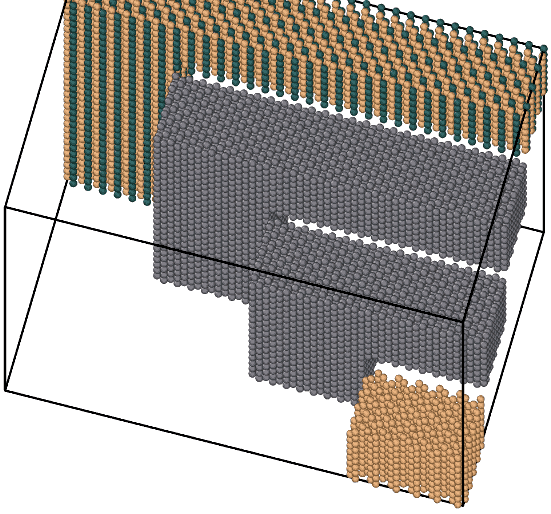
\includegraphics[width=1\textwidth]{images/lattice-full.png}
    \captionof{figure}{Simulation data saved with full lattice}
    \label{fig-save-lattice-full}
  \end{minipage}
  \qquad
  \begin{minipage}{.45\textwidth}
    \centering
    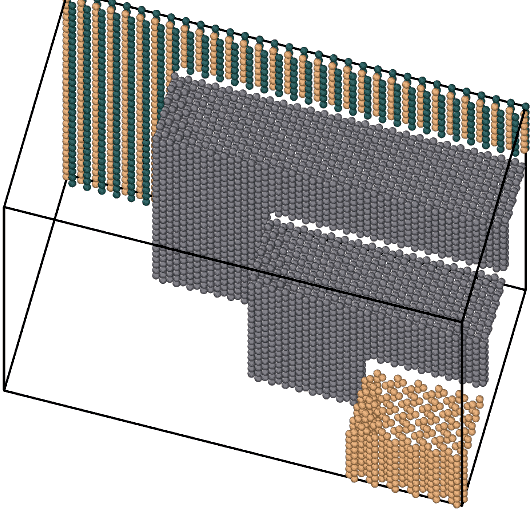
\includegraphics[width=1\textwidth]{images/lattice-near-gas.png}
    \captionof{figure}{Simulation data saved with lattice atoms near the solid-gas cell interface}
    \label{fig-save-lattice-near-gas}
  \end{minipage}
\end{figure}
